\section*{命题、联结词与命题公式}

\textbf{命题}:非真即假/可明确判真假的陈述句\\
·\textbf{悖论}:[我正在撒谎]既不为真也不为假\\
· [长方形是正方形]既可为真也可为假

\textbf{真值}:命题的判断结果,只取真或假两个值

\textbf{真命题/假命题}:真值为真/假的命题

\textbf{命题符号化}:将命题抽象为取值为0or1的$p$,$q$...

\textbf{简单命题(原子命题)}:不能被分解成更简单的命题的命题

\textbf{复合命题}:由简单命题通过联结词联结而成的命题

·其真假完全由构成它的简单命题的真假决定

·简单命题和复合命题的划分是相对的

\textbf{否定式}:复合命题“非$p$”称作$p$的否定式,$\neg p$

\textbf{否定联结词}:$\neg$,规定$\neg p$为真当且仅当$p$为假

\textbf{合取式}:复合命题“$p$并且$q$”称为$p$与$q$的合取式,记作$p \wedge q$

\textbf{合取联结词}:$\wedge$,规定$p \wedge q$为真当且仅当$p$与$q$同时为真

\textbf{析取式}:复合命题“$p$或$q$”称作$p$与$q$的析取式,记作$p \vee q$

\textbf{析取联结词}:$\vee$,规定$p \vee q$为假当且仅当$p$与$q$同时为假

·\textbf{相容或与相斥或}:$\vee$与$\bar{\vee}$, $\bar{\vee}$为真要满足$p, q$不同时为真;不能看见$p$或$q$就转化为$p \vee q$

\textbf{蕴涵式}:复合命题“如果$p$,则$q$”称为$p$与$q$的蕴涵式,记作$p \rightarrow q$,并称$p$是前件,$q$是后件

·例子:如果$p$则$q$;$q$每当$p$;$p$仅当$q$;只有$q$才$p$;除非$q$才$p$;除非$q$,否则$\lnot p$

\textbf{蕴涵联结词}:$\rightarrow$,规定$p \rightarrow q$为假当且仅当$p$为真而$q$为假($p \le q$)

\textbf{等价式}:复合命题“$p$当且仅当$q$”称作$p$与$q$的等价式,记作$p \leftrightarrow q$

\textbf{等价联结词}:$\leftrightarrow$,规定$p \leftrightarrow q$为真当且仅当$p$与$q$同时为真或同时为假

\textbf{命题常量}:一个特定的命题,真值确定

\textbf{命题变量/项/元}:一个没有赋予具体内容的命题,真值可变

\textbf{命题公式(命题形式)}:由命题变元和联结词按以下规则组成的符号串\\
1.任何命题变元都是命题公式,称为原子命题公式\\
2.如果$A$是命题公式,则$\lnot A$也是命题公式\\
3.如果$A$、$B$是命题公式,则$(A \vee B)$、$(A \wedge B)$、$(A \rightarrow B)$和$(A \leftrightarrow B)$都是命题公式\\
只有有限次地应用(1)—(3)构成的符号串才是命题公式\\
命题公式定义是归纳定义,而不是循环定义,(1)是奠基,(2)、(3)是归纳步骤

·公式中的0, 1看作可看作$(A \wedge (\lnot A))$、$(A \vee (\lnot A))$

\textbf{约定运算顺序}

省略命题公式最外层括号;$\lnot$的优先级高于其它的联结词,只作用于紧随其后的命题变元;相同联结词可以省略括号;优先级:(否定) > (合取、析取) > (蕴涵、等价)

\textbf{赋值(解释)}:设$p_1, p_2, \ldots, p_n$是出现在命题公式$A$中的所有命题变元,对序列$p_1, p_2, \ldots, p_n$指定的的任一真值序列,称为对$A$的一个赋值

\textbf{成真/假赋值}:若$p_1, p_2, \ldots, p_n$的一个赋值使$A$为真/假,则称此赋值为$A$的一个成真/假赋值

\textbf{重言式(永真式)/矛盾式(永假式)}:$A$关于其中出现的命题变元的所有赋值均为成真/假赋值

\textbf{可满足式}:$A$对于其中出现的命题变元的某个赋值为成真赋值

\textbf{哑元}:未出现在$A$中的命题变元,$A$取值与哑元取值无关

\section*{等值式与范式}

\textbf{等值式}:若$A, B$构成的等价式$A \leftrightarrow B$为重言式,则称$A$与$B$等值,记作$A \Leftrightarrow B$,并称$A \Leftrightarrow B$是等值式;等值是一种等价关系

\textbf{文字}:命题变项及其否定的统称

\textbf{简单析/合取式}:仅由有限个文字构成的析/合取式

\textbf{范式}:由有限个简单合/析取式的\textbf{析/合}取构成的命题公式称作\textbf{析/合}取范式;析取范式与合取范式统称作范式

·简单合(析)取式既是析取范式又是合取范式

\textbf{极小/大项}:以含$p, q, r$的情况为例\\
·$m_1 = \lnot p \wedge \lnot q \wedge r$(下标=成真赋值)\\
·$M_1 = p \vee q \vee \lnot r$(下标=成假赋值)

\textbf{主析/合取范式}:所有简单合/析取式都是极小/大项的析/合取范式

\textbf{n元真值函数}:$F:\{0,1\}^n \rightarrow \{0,1\}$

\textbf{联结词的完备集S}:仅由$S$中的联结词构成的公式可表示所有真值函数

\textbf{与非、或非}:$\uparrow$表示与非,$\downarrow$表示或非

\section*{命题逻辑推理}
	
\textbf{推理形式}:由前提 $\alpha_1$, $\alpha_2$, $\cdots$, $\alpha_n$ 推出结论 $\beta$

\textbf{推理正确(有效)}:如果对 $\alpha_1$, $\cdots, \alpha_n$, $\beta$ 中出现的命题变元的任意赋值,若 $\alpha_1 \land \alpha_2 \land \cdots \land \alpha_n$ 为假,或若 $\alpha_1 \land \alpha_2 \land \cdots \land \alpha_n$ 为真时 $\beta$ 亦真,则称推理 "$\alpha_1$, $\alpha_2$, $\cdots$, $\alpha_n$ 推出 $\beta$" 有效,否则是不合理(无效)的。

·注:若出现\textbf{前提为真结论为假}的情况则推理无效!

\textbf{逻辑蕴涵}$\Rightarrow$: 前提:$\alpha_1$, $\alpha_2$, $\cdots$, $\alpha_n$ 结论:$\beta$ 推理正确记为 $\alpha_1 \land \alpha_2 \land \cdots \land \alpha_n \Rightarrow \beta$

·$A \rightarrow B$ 是命题公式,$A \Rightarrow B$ 表示两个命题公式之间的逻辑蕴涵关系

\textbf{自然推理系统P}:\\
·字母表:命题变元、联结词、括号逗号\\
·命题公式:(见上)\\
·推理规则:(见定理)

\section*{一阶谓词逻辑}

\textbf{个体}:独立存在的客体\\
·个体常元:表示具体事物,$a, b, c, \ldots$\\
·个体变元:抽象事物(不确定具体哪个) $x, y, z, \ldots$

\textbf{个体域}:个体变元的取值范围\\
·全总个体域:由宇宙间一切事物组成的个体域

\textbf{谓词}:表示个体性质或彼此之间关系$F, G, H, \ldots$\\
·谓词常元:表示具体性质或关系\\
·谓词变元:表示抽象的或泛指的性质或关系

\textbf{n元谓词}:含 $n$ 个【个体变元】的谓词,是定义在个体域上,值域为 $\{0,1\}$ 的 $n$ 元函数\\
·一元谓词:表示事物的性质\\
·多元谓词:表示事物之间的关系\\
·0元谓词:不含个体变元的谓词,就是命题常项或命题变项

注:将 $n$ 元谓词中的个体变元都用个体域中具体的个体取代后,就成为一个命题

\textbf{量词}:表示数量的词\\
\textbf{全称量词 $\forall$}:自然语言中“所有的”、“一切的”、“任意的”、“每一个”、“都”等的统称。 $\forall x$ 个体域中的所有个体; $\forall x F(x)$ 个体域里的所有 $x$ 都有性质 $F$\\
\textbf{存在量词 $\exists$}:自然语言中“有一个”、“至少有一个”、“存在着”、“有的”等的统称。 $\exists x$ 存在个体域里的 $x$; $\exists x F(x)$ 在个体域里存在 $x$ 具有性质 $F$

\textbf{有限域下的公示表示法}(无穷集下无)

·$\forall x P(x) = P(1) \land P(2) \land \ldots \land P(k)$:对任意的 $x$,$P(x)$ 均成立,合取联结词的推广

·$\exists x P(x) = P(1) \lor P(2) \lor \ldots \lor P(k)$:有一个 $x$ 使得 $P(x)$ 成立,析取联结词的推广

\textbf{特性谓词 $M(x)$}:用于将个体变元局限在满足该谓词代表的性质或关系的范围之内

\textbf{命题符号化}应注意以下几点:

·两个基本公式:$\forall x (M(x) \rightarrow F(x))$,个体域中所有有性质 $M$ 的个体都有性质 $F$;$\exists x (M(x) \land G(x))$,个体域中存在有性质 $M$ 同时有性质 $G$ 的个体

·同一命题在不同个体域中符号化形式可能不同

·同一命题在不同个体域中真值可能不同

·命题中表示性质和关系的谓词,分别符号化为一元和 $n$ 元谓词

·多个量词出现时,仅同类量词可交换顺序

·定理:$(\exists x)(\forall y) P(x,y) \Rightarrow (\forall y)(\exists x) P(x,y)$

\textbf{函数符号}:个体域$D$上,$n$元函数符号$f(x_1, \dots, x_n)$是$D^n\rightarrow D$的函数(与谓词差异在于值域)

\textbf{一阶语言 $\mathcal{L}$ 的字母表}

非逻辑符号:所描述的特定对象中的符号\\
·个体常元:$a, b, c, \ldots, a_{i}, b_{i}, c_{i}, i \geq 1$\\
·函数符号:$f, g, h, \ldots, f_{i}, g_{i}, h_{i}, \ldots, i \geq 1$\\
·谓词符号:$F, G, H, \ldots, F_{i}, G_{i}, H_{i}, i \geq 1$
	
逻辑符号:逻辑系统中的符号\\
·个体变元:$x, y, z, \ldots, x_{i}, y_{i}, z_{i}, \ldots, i \geq 1$\\
·量词符号:$\forall, \exists$\\
·联结词符号:$\neg, \land, \vee, \rightarrow, \leftarrow$\\
·括号与逗号:(), \, 

\textbf{$\mathcal{L}$ 的项}\\
1. 个体常元和个体变元是项\\
2. 若 $\varphi (x_{1}, x_{2}, \ldots, x_{n})$ 是 $n$ 元函数,$t_{1}, t_{2}, \ldots, t_{n}$ 是任意的 $n$ 个项,则 $\varphi (t_{1}, t_{2}, \ldots, t_{n})$ 是项\\
3. 所有的项都是有限次使用 (1), (2) 得到的

\textbf{原子公式}:设 $R(x_1, x_2, \ldots, x_n)$ 是 $\mathcal{L}$ 任意的 $n$ 元谓词,$t_1, t_2, \ldots, t_n$ 是 $\mathcal{L}$ 的任意 $n$ 个项,则称 $R(t_1, t_2, \ldots, t_n)$ 是原子公式

\textbf{定义 $\mathcal{L}$ 的合式公式}\\
1. 原子公式是合式公式\\
2. 若 $A$ 是合式公式,则 $(\neg A)$ 也是合式公式\\
3. 若 $A$, $B$ 是合式公式,则 $(A \land B), (A \vee B), (A \rightarrow B), (A \leftrightarrow B)$ 也是合式公式\\
4. 若 $A$, $B$ 是合式公式,则 $(\forall x)A, (\exists x)A$ 也是合式公式

·项是(复合)个体;(原子)公式是完整的判断

注1:一阶语言中的原子公式取代了命题公式

注2:所有一阶语言中都含有相同的逻辑符号,但所含的非逻辑符号不一定相同

注3:在定义中没有要求个体$x$一定要在$A$中出现,$(\forall x_1)F(x_1,x_2),(\forall x_3)F(x_1,x_2)$都是公式

注4:$L$中至少有一个谓词符号,否则$L$生成的一阶语言中没有公式

\textbf{括号省略规则}\\
1.省略公式最外层的括号\\
2.联结词$\lnot$的优先级高于其他联结词,可以去掉($\neg\alpha$)中的外层括号\\
3.$\forall x, \exists x$优先级高于所有联结词,将$(\forall x)\alpha, (\exists x)\alpha$记作$\forall x \alpha, \exists x \alpha$;$(\forall x_1) \cdots (\forall x_n)\alpha$简记为$\forall x_1 \cdots \forall x_n \alpha$,$(\exists x_1) \cdots (\exists x_n)\alpha$简记为$\exists x_1 \cdots \exists x_n \alpha$

\textbf{辖域}:公式 $\forall x A$ 和 $\exists x A$ 中,称 $x$ 为 \textbf{指导变元},$A$ 为相应量词的 \textbf{辖域}

\textbf{约束出现}:在 $\forall x$ 和 $\exists x$ 的辖域中(包括 $\forall x$ 和 $\exists x$ 中的 $x$),$x$ 的所有出现称为约束出现,$A$ 中不是约束出现的其他变元称为 \textbf{自由出现}

\textbf{约束变元}:设个体变元 $x$ 在公式 $\alpha$ 中出现,若 $x$ 在 $\alpha$ 中的所有出现【均】为约束出现,则称 $x$ 为 $\alpha$ 的约束变元;否则称为\textbf{自由变元}


\textbf{闭式}:设 $A$ 是任意的公式,若 $A$ 中不含自由出现的个体变元,则称 $A$ 为封闭的公式,简称闭式

·要将含 $r$ 个自由出现的个体变元的公式变成闭式,至少需要加上 $r$ 个量词

\textbf{解释与赋值}

·设一阶语言 $\mathcal{L}$ 个体常元集 $\{ a_{i} \}$,函数符号集 $\{ f_{i} \}$,谓词符号集 $\{ F_{i} \}$,$\mathcal{L}$ 的解释 $I$ 由下面 4 部分组成:\\
1. 非空个体域 $D_I$\\
2. 对每一个个体常元 $a_i, \bar{a_{i}} \in D_I$,称作 $a_{i}$ 在 $I$ 中的解释\\
3. 对每一个函数符号 $f_{i}$,设其为 $m$ 元的,$\bar{f_{i}}$ 是 $D_I$ 上的 $m$ 元函数,称作 $\bar{f_{i}}$ 在 $I$ 中的解释\\
4. 对每一个谓词符号 $F_{i}$,设其为 $n$ 元的,$\bar{F_{i}}$ 是一个 $n$ 元谓词,称作 $F_{i}$ 在 $I$ 中的解释

·$I$下的\textbf{赋值} $\sigma$:对每一个【自由出现】的个体变元 $x$ 指定个体域中的一个值 $\sigma(x)$\\
\fontsize{4pt}{5pt}
注1:任何公式在给定的解释和赋值下都是命题\\
注2:闭式在任何解释下都变成命题(无需赋值)

\fontsize{6pt}{7pt}
\textbf{永真式(逻辑有效式)}:无成假解释和赋值\\
\textbf{矛盾式(永假式)}:无成真解释和赋值\\
\textbf{可满足式}:至少有一个成真解释和赋值

\textbf{代换实例}:
设 $A_0$ 是含命题变项 $p_1, p_2, \ldots, p_n$ 的命题公式,$A_1, A_2, \ldots, A_n$ 是 $n$ 个谓词公式,用 $A_i$ 处处代替 $A_0$ 中的 $p_i (1 \leq i \leq n)$,所得公式 $A$ 称为 $A_0$ 的代换实例。例如,$F(x) \rightarrow G(x)$, $\forall x F(x) \rightarrow \exists y G(y)$ 都是 $p \rightarrow q$ 的代换实例

\textbf{等值式}:设 $A, B$ 是一阶逻辑中任意两个公式,若 $A \leftrightarrow B$ 是永真式,则称 $A$ 与 $B$ 等值,记作 $A  \Leftrightarrow B$,并称 $A  \Leftrightarrow B$ 为等值式

\textbf{前束范式}:一阶逻辑公式 $A$ 具 $Q_{1} x_{1} \ldots Q_{k} x_{k} B$ 的形式。其中 $Q_{i} = \forall$ 或 $\exists$,$B$(母式/基式)不含量词

\textbf{推理正确(有效)}:在一阶逻辑中,从前提 $A_1, \ldots, A_k$ 推出结论 $B$ 正确,若 $A_{1} \land \ldots \land A_{k} \rightarrow B$ 为永真式,记作 $A_{1} \land \ldots \land A_{k} \Rightarrow B$,否则称推理不正确

\textbf{自然推理系统 $N_L$}
一阶逻辑自然推理系统包括:\\
1. 字母表:同一阶语言字母表\\
2. 合式公式(谓词公式):(见上)\\
3. 推理规则:(见定理)


\hrule

\section*{等值式与范式定理}

\textbf{交换律} $A \vee B  \Leftrightarrow B \vee A, A \land B  \Leftrightarrow B \land A, A \leftrightarrow B  \Leftrightarrow B \leftrightarrow A$

\textbf{结合律} $(A \vee B) \vee C  \Leftrightarrow A \vee (B \vee C)$, $(A \land B) \land C  \Leftrightarrow A \land (B \land C)$, $(A \leftrightarrow B) \leftrightarrow C  \Leftrightarrow A \leftrightarrow (B \leftrightarrow C)$

\textbf{分配律} $A \rightarrow (B \rightarrow C)  \Leftrightarrow (A \rightarrow B) \rightarrow (A \rightarrow C)$

$A \vee (B \land C)  \Leftrightarrow (A \vee B) \land (A \vee C)$,与或可互换

\textbf{双重否定律} $A  \Leftrightarrow \neg \neg A$

\textbf{德摩根律} $\neg (A \vee B)  \Leftrightarrow \neg A \land \neg B, \neg (A \land B)  \Leftrightarrow \neg A \vee \neg B$

\textbf{幂等律} $A \vee A \Leftrightarrow A, A \land A \Leftrightarrow A, A \rightarrow A \Leftrightarrow 1, A \leftrightarrow A  \Leftrightarrow 1$

\textbf{吸收率} $A \vee (A \land B)  \Leftrightarrow A, A \land (A \vee B)  \Leftrightarrow A$

\textbf{零律} $A \vee 1  \Leftrightarrow 1, A \land 0 \Leftrightarrow 0, A \rightarrow 1 \Leftrightarrow 1, 0 \rightarrow A \Leftrightarrow 1$

\textbf{同一律} $A \vee 0  \Leftrightarrow A, A \land 1  \Leftrightarrow A, A \rightarrow 0  \Leftrightarrow \lnot A, 0 \leftrightarrow A  \Leftrightarrow \lnot A$

\textbf{排中律} $A \vee \neg A  \Leftrightarrow 1$

\textbf{矛盾律} $A \land \neg A  \Leftrightarrow 0$

\textbf{蕴涵等值式} $A \rightarrow B  \Leftrightarrow \neg A \vee B$

\textbf{等价等值式} $A \leftrightarrow B  \Leftrightarrow (A \rightarrow B) \land (B \rightarrow A)$

\textbf{假言易位} $A \rightarrow B  \Leftrightarrow \neg B \rightarrow \neg A$

\textbf{等价否定等值式} $A \leftrightarrow B  \Leftrightarrow \neg A \leftrightarrow \neg B$

\textbf{归谬律} $(A \rightarrow B) \land (A \rightarrow \neg B)  \Leftrightarrow \neg A$

\textbf{其他} $A \rightarrow \neg A  \Leftrightarrow \neg A, \neg A \rightarrow A  \Leftrightarrow A, A \leftrightarrow \neg A  \Leftrightarrow 0$

$A \rightarrow (B \rightarrow C)  \Leftrightarrow (A \land B) \rightarrow C  \Leftrightarrow B \rightarrow (A \rightarrow C)$

$A \leftrightarrow B  \Leftrightarrow (A \land B) \vee (\neg A \land \neg B)  \Leftrightarrow (\neg A \vee B) \land (A \vee \neg B)$

$(A \rightarrow C) \land (B \rightarrow C)  \Leftrightarrow (A \vee B) \rightarrow C$

\textbf{置换规则}:设 $\phi(A)$ 是含公式 $A$ 的公式,用公式 $B$ 置换 $\phi(A)$ 中的 $A$,得公式 $\phi(B)$,如果 $A  \Leftrightarrow B$,则 $\phi(A)  \Leftrightarrow \phi(B)$

\textbf{证明等值式}:真值表法/等值演算

\textbf{证明不等值式}:真值表法/观察出一个不等值的赋值/先等值演算再观察

·一个简单\textbf{析取式是重言式}当且仅当它同时含某个命题变项及它的否定式

·一个简单\textbf{合取式是矛盾式}当且仅当它同时含某个命题变项及它的否定式

·一个析取范式是矛盾式当且仅当它的\textbf{每个简单合取式}都是\textbf{矛盾式}

·一个合取范式是重言式当且仅当它的\textbf{每个简单析取式}都是\textbf{重言式}

\textbf{范式存在定理}:任一命题公式都存在与之等值的析取范式与合取范式

·方法:利用蕴涵等值式和等价等值式消去;利用双重否定式和德摩根率将$\lnot$消去或内移;分配律

\textbf{一些联结词的完备集}:$\{\lnot, \wedge\}, \{\lnot, \vee\}, \{\lnot, \rightarrow\}, \{\uparrow\}, \{\downarrow\}$

·证明:从主析取出发得$\{\lnot, \wedge, \vee\}$,其他通过符号间的表示

·不考虑与非、或非,2元素有3个完备,3元素有6个完备(含$\lnot$即可),4元素有4个完备

\section*{命题逻辑的推理定律}

\textbf{$\Rightarrow$的基本性质}\\
·若 $A \Rightarrow B$,$A$ 为重言式,则 $B$ 也是重言式\\
·若 $A \Rightarrow B$,$B \Rightarrow A$ 同时成立,必有 $A  \Leftrightarrow B$\\
·若 $A \Rightarrow B$,$B \Rightarrow C$,则 $A \Rightarrow C$\\
·若 $A \Rightarrow B$,$A \Rightarrow C$,则 $A \Rightarrow B \land C$\\
·若 $A \Rightarrow C$,$B \Rightarrow C$,则 $A \lor B \Rightarrow C$

\textbf{证明推理公式 $A \Rightarrow B$ 的方法}

·真值表法;直观解释法【关注前提为真结论为假】

·主析取/合取范式法;等值演算法【根据充要条件 $A \rightarrow B$ 为永真式或$A \land \neg B$ 为矛盾式】

·若 $\neg B \Rightarrow \neg A$,则 $A \Rightarrow B$

\textbf{附加律}:$A \Rightarrow (A \vee B)$

\textbf{化简律}:$(A \land B) \Rightarrow A$

\textbf{假言推理}:$(A \rightarrow B) \land A \Rightarrow B$

\textbf{拒取式}:$(A \rightarrow B) \land \neg B \Rightarrow \neg A$

\textbf{析取三段论}:$(A \vee B) \land \neg A \Rightarrow B$, $(A \vee B) \land \neg B \Rightarrow A$

\textbf{假言三段论}:$(A \rightarrow B) \land (B \rightarrow C) \Rightarrow (A \rightarrow C)$

\textbf{等价三段论}:$(A \leftrightarrow B) \land (B \leftrightarrow C) \Rightarrow (A \leftrightarrow C)$

\textbf{构造性二难}:$(A \rightarrow B) \land (C \rightarrow D) \land (A \vee C) \Rightarrow (B \vee D)$

\textbf{构造性二难(特殊形式)}:$(A \rightarrow B) \land (\neg A \rightarrow B) \Rightarrow B$

\textbf{破坏性二难}:$(A \rightarrow B) \land (C \rightarrow D) \land (\neg B \vee \neg D) \Rightarrow (\neg A \vee \neg C)$

\textbf{推理定律 10}:$\neg A \Rightarrow (A \rightarrow B)$;$B \Rightarrow (A \rightarrow B)$;$\neg (A \rightarrow B) \Rightarrow A$;$\neg (A \rightarrow B) \Rightarrow \neg B$

\textbf{推理定律 11}:$(B \rightarrow C) \Rightarrow (A \rightarrow B) \rightarrow (A \rightarrow C)$;$(B \rightarrow C) \Rightarrow (A \vee B) \rightarrow (A \vee C)$

\textbf{利用自然推理系统P构造推理的证明}:

·\textbf{推理规则}:前提引入规则、结论引入规则、置换规则、合取引入规则($A, B \Rightarrow A \land B$)

1.\textbf{直接证明法}

2.\textbf{附加前提证明法}:如果推理的结构有如下形式:$(A_1 \land A_2 \land \ldots \land A_k) \rightarrow (C \rightarrow B)$,则可以将结构改写为:$(A_1 \land A_2 \land \ldots \land A_k \land C) \rightarrow B$[\textbf{附加前提引入}]

3.\textbf{归谬法}:引入结论的否定作为附加前提,若能推出矛盾式,则此推理有效[\textbf{结论否定引入}]

4.\textbf{消解证明法}:把【结论的否定】及【前提】都化成合取范式,以这些合取范式中的【简单析取式】为前提,仅用归结规则规则构造证明推出0

·归结规则:$(A \vee B) \land (\lnot A \vee C) \Rightarrow B \vee C$

\section*{一阶谓词逻辑等值式}

1.命题逻辑等值式的代换实例都是一阶逻辑的等值式

2.1\textbf{量词否定等值式} $A(x)$ 是含 $x$ 自由出现的公式:
\begin{enumerate}
	\item $\neg \forall x A(x)  \Leftrightarrow \exists x \neg A(x)$
	\item $\neg \exists x A(x)  \Leftrightarrow \forall x \neg A(x)$
\end{enumerate}

2.2\textbf{量词辖域收缩与扩张等值式}:$A(x)$ 是含 $x$ 自由出现的公式;$B$ 中不含 $x$ 的自由出现:
\begin{enumerate}
	\item$\forall x (A(x) \vee B) \Leftrightarrow \forall x A(x) \vee B$
	\item$\forall x (A(x) \land B) \Leftrightarrow \forall x A(x) \land B$
	\item$\forall x (A(x) \rightarrow B) \Leftrightarrow \exists x A(x) \rightarrow B$
	\item$\forall x (B \rightarrow A(x)) \Leftrightarrow B \rightarrow \forall x A(x)$

	\item$\exists x (A(x) \vee B) \Leftrightarrow \exists x A(x) \vee B$
	\item$\exists x (A(x) \land B) \Leftrightarrow \exists x A(x) \land B$
	\item$\exists x (A(x) \rightarrow B) \Leftrightarrow \forall x A(x) \rightarrow B$
	\item$\exists x (B \rightarrow A(x)) \Leftrightarrow B \rightarrow \exists x A(x)$
\end{enumerate}

2.3\textbf{量词分配等值式} $A(x)B(x)$ 是含 $x$ 自由出现的公式:
\begin{enumerate}
	\item $\forall x (A(x) \land B(x))  \Leftrightarrow \forall x A(x) \land \forall x B(x)$
	\item $\exists x (A(x) \lor B(x))  \Leftrightarrow \exists x A(x) \land \exists x B(x)$
\end{enumerate}

· $\forall$ 对 $\vee$ 无分配律,$\exists$ 对 $\land$ 无分配律!

3.1\textbf{置换规则}:设 $\Phi(A)$ 是含公式 $A$ 的公式,$\Phi(B)$ 是用公式 $B$ 取代 $\Phi(A)$ 中所有 $A$ 所得到的公式,若 $A  \Leftrightarrow B$,则 $\Phi(A)  \Leftrightarrow \Phi(B)$

3.2\textbf{换名规则}:\\
·约束变元:【指导变元】及其【辖域中的约束出现】一起换成该量词辖域中没出现过的变元\\
·自由变元:公式中自由变元的所有自由出现一起换(且不允许在原公式中以约束形式出现)

\textbf{前束范式存在定理}:一阶逻辑中的任何公式都存在与之等值的前束范式,但其前束范式并不唯一

\textbf{化前束范式的方法}:设 $G$ 是任一公式\\
1. 消去公式中包含的联结词 $\rightarrow$(非必要), $\leftrightarrow$\\
2. 反复使用德摩根律将 $\neg$ 内移\\
3. 使用分配等值式将量词左移\\
4. (不能使用分配律时)先易名后辖域扩张

\section*{一阶逻辑的推理定律}

1. 命题逻辑推理定律的代换实例\\
·例:$\forall x F(x) \land \forall y G(y) \Rightarrow \forall x F(x)$(化简律)

2. 常用的重要推理定律:
\begin{enumerate}
	\item $\forall x A(x) \Rightarrow \exists x A(x)$
	\item $\forall x A(x) \vee \forall x B(x) \Rightarrow \forall x (A(x) \vee B(x))$~仅单向!
	\item $\exists x (A(x) \land B(x)) \Rightarrow \exists x A(x) \land \exists x B(x)$~仅单向!
	\item $\forall x (A(x) \rightarrow B(x)) \Rightarrow \forall x A(x) \rightarrow \forall x B(x)$
	\item $\forall x (A(x) \rightarrow B(x)) \Rightarrow \exists x A(x) \rightarrow \exists x B(x)$
	\item $\forall x (A(x) \leftrightarrow B(x)) \Rightarrow \forall x A(x) \leftrightarrow \forall x B(x)$
	\item $\forall x (A(x) \leftrightarrow B(x)) \Rightarrow \exists x A(x) \leftrightarrow \exists x B(x)$
\end{enumerate}

3. 含有多个量词的公式:

\begin{figurehere}
	\centering
	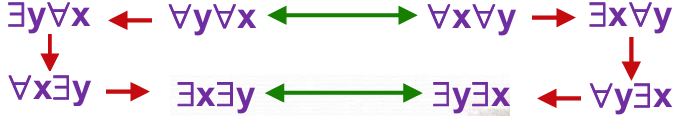
\includegraphics[width=0.8\linewidth]{image01}
	\label{fig:image01}
\end{figurehere}


4. 量词的消去/引入规则:
设 $x, y$ 为个体变元符号,$c$ 为个体常元,【$y$ 不在 $A(x)$ 中约束出现】
\begin{enumerate}
	\item \textbf{$\forall -$}:$(\forall x) A(x) \Rightarrow A(y), (\forall x) A(x) \Rightarrow A(c)$
	\item \textbf{$\forall +$}:$A(y) \Rightarrow (\forall x) A(x)$ 限制:$x$ 不在 $A(y)$ 中约束出现[重名引起混乱]
	\item \textbf{$\exists -$}:$(\exists x) A(x) \Rightarrow A(c)$ 限制:$(\exists x) A(x)$ 中无自由变元[否则$x$依赖于自由变元],且不含 $c$
	\item \textbf{$\exists +$}:$A(c) \Rightarrow (\exists x) A(x)$ 限制:$x$ 不出现于 $A(c)$
\end{enumerate}

\textbf{一阶自然推理系统$N_L$构造推理的证明}:\\
\fontsize{5.9pt}{6pt}
·推理规则:$12$条命题逻辑推理规则、$\forall -, \forall +, \exists -, \exists +$\\
\fontsize{6pt}{7pt}
·推理方法:\\
1. 前提引入规则和结论引入规则\\
2. 如果结论是以蕴涵形式(或析取形式)给出,可使用附加前提证明法\\
3. 若需消去量词,用全称量词消去规则和存在量词消去规则\\
4. 当所要求的结论可能被定量时,用全称量词引入规则和存在量词引入规则将量词加入\\
5. 对消去量词的公式或公式中不含量词的子公式,用命题演算中的基本等价公式和基本推理定律\\
6. 对含有量词的公式可以用谓词中的基本等价公式和基本推理定律

注1.如公式中既要消去存在量词又要消去全称量词,且所选用的个体是同一个符号,则必须 \textbf{先消去存在量词再消去全称量词}

\begin{figurehere}
	\centering
	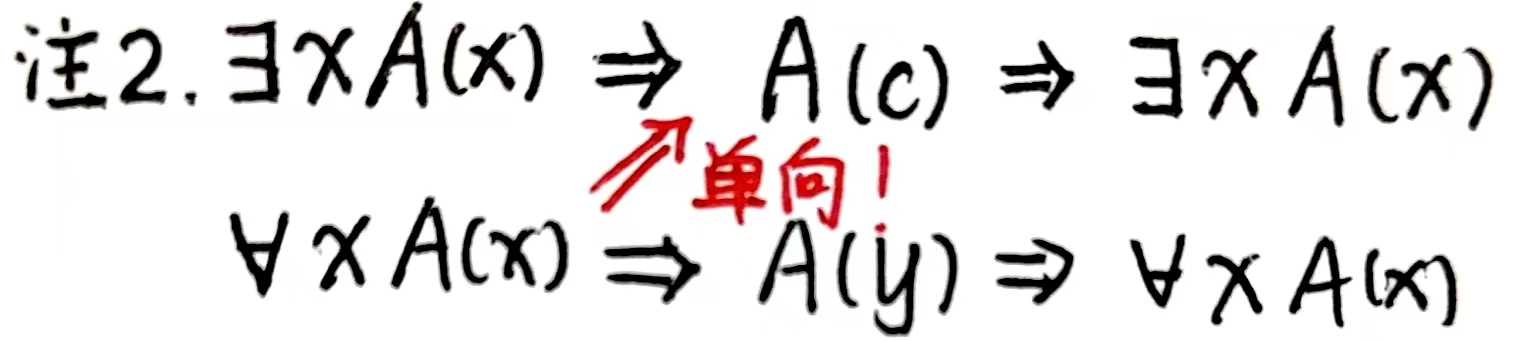
\includegraphics[width=0.7\linewidth]{image02}
	\label{fig:image02}
\end{figurehere}

注3.有两个含有存在量词的公式,当消去存在量词时,不能选用同样的一个常量符号来取代两个公式中的变元,而 \textbf{应用不同的常量符号}

注4.使用 $\forall +, \forall -, \exists +, \exists -$ 时,此量词必须位于整个公式的最前端,且它的辖域为其后的整个公式
